\subsection{Plot the concept}
\begin{figure}[h!]
    \centering
    \includegraphics[width=0.8\textwidth]{fig/TWFE_fig.png}
    \caption{A failure of simply using the two way fixed effect on staggered treatment effect}
    \label{fig:TWFE_1}
\end{figure}

See figure \ref{fig:TWFE_1}. The purpose of DiD is to extract the trend 
of the treated in a way that the counterfactual outcome can be obtained. 
The TWFE, however, takes the treated (the orange line after $T_1$) as the controlled group, 
causing the DiD on the blue cohort to actually look to have a downward effect.

\subsection{Simulation}

Referring to an excellent article written by Callaway and Sant’Anna (2022), 
I replicated a simplified version of the concept \footnote{https://cran.r-project.org/web/packages/did/vignettes/TWFE.html}.

The data generating process is as follow
\begin{equation*}
    Y_{i,t,g} = (2020-g) + \alpha_i + \alpha_{t,g} + \tau_{i,t} + \epsilon_{i,t} 
\end{equation*}
where $i$ is the unit, $t$ is the year, and $g$ is the group. Each unit belongs to a state. 
There are 40 states in this data generating process, 
each randomly assigned to one of the treated-year in the group $\{2005, 2010, 2015, 2020\}$. 
Therefore each unit corresponds to one of the group, and hence is treated in one of the year above.
The fixed effects are defined as follow 
\begin{align*}
    \alpha_i &\sim \mathcal{N}(0.2 state, 1) \\
    \alpha_t &\sim 0.1(t-g) + \epsilon^{FE}_{t} \\
    \epsilon^{FE}_{t} &\sim \mathcal{N}(0,1)\\
    \tau_{i,t} &= \mu (t - g + 1) \one\{t \ge g\}\\
    \epsilon_{i,t} &\sim \mathcal{N}(0,\frac{1}{4}) 
\end{align*}

The time series data is shown in figure~\ref{fig:mc_result}. Here the treatment effect $\mu$ is set to be $2$.

\begin{figure}[t]
    \centering
    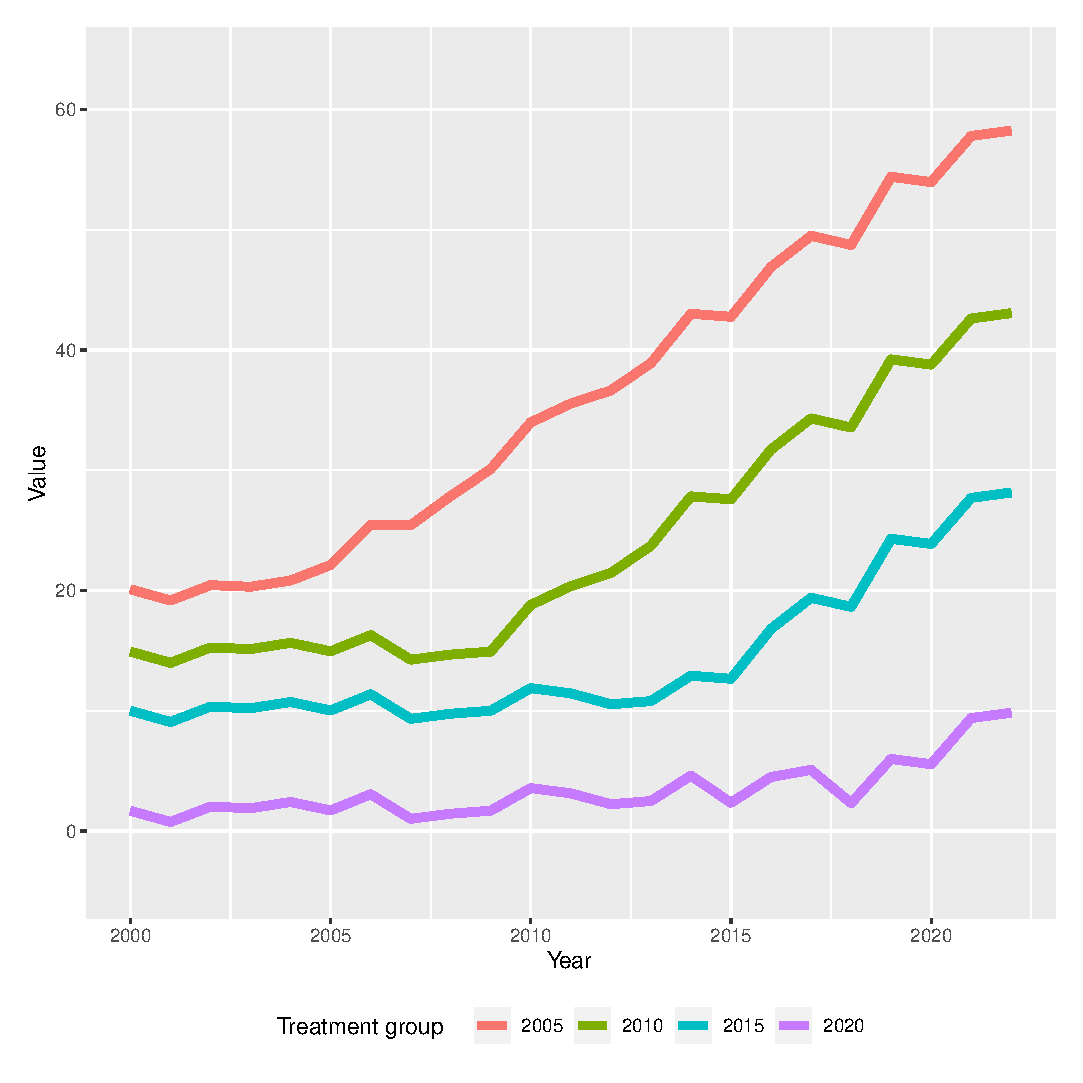
\includegraphics[width = 0.7\textwidth]{fig/sim_twfe.eps}
    \caption{Data for Monte-Carlo simulation }
    \label{fig:mc_result}
\end{figure}

Note that $ \alpha_t$ is a cohort specific parallel time-trend, 
the expected value of time fixed effect for each group will then be set to 0 when they are treated. 

We then estimate the following TWFE
\begin{equation*}
    Y_{i,t} = \alpha_i + \alpha_t + D_{it}\beta_{TWFE} + \epsilon_{it}
\end{equation*}

The result is shown in figure \ref{fig:TWFE_coef}
\begin{figure}
    \centering
    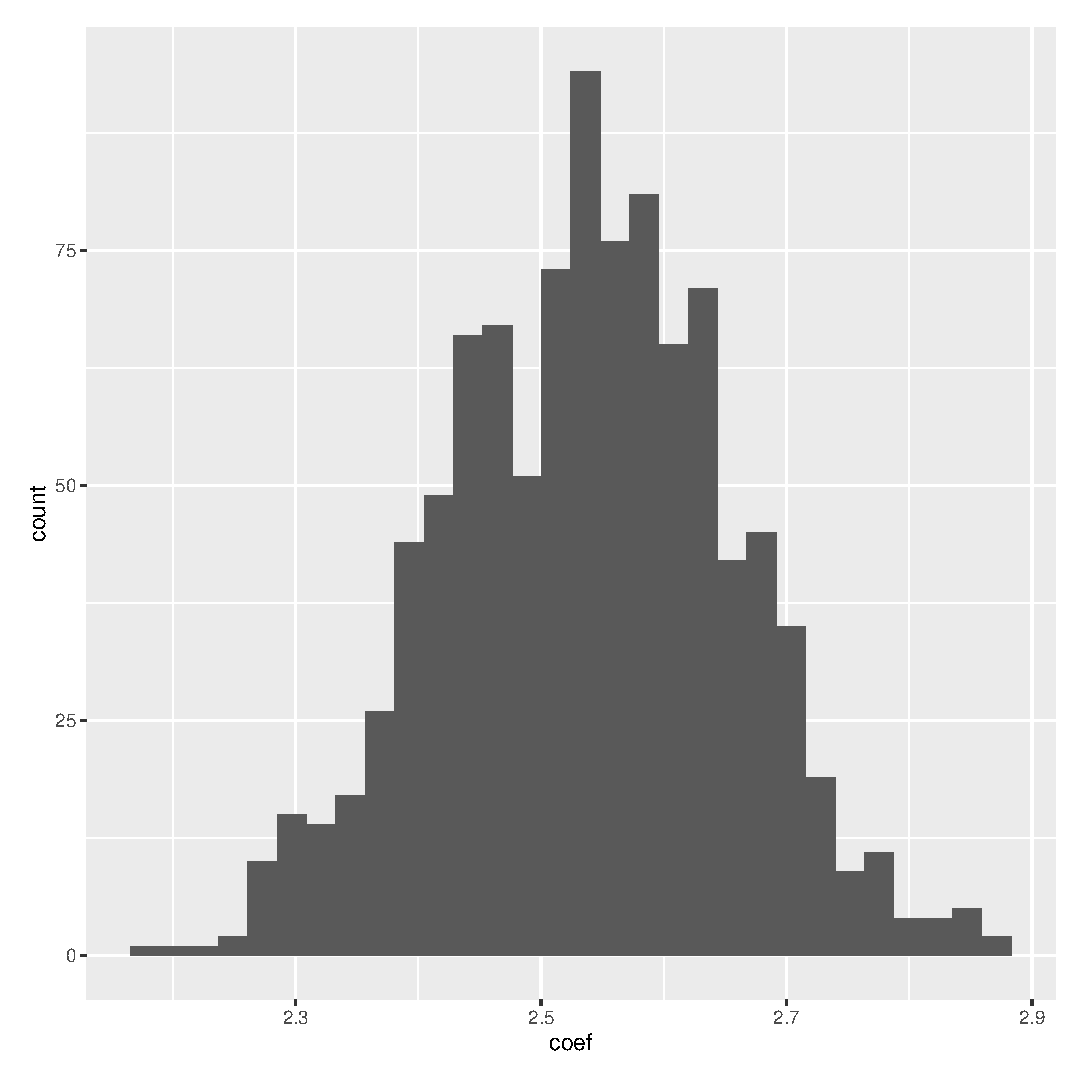
\includegraphics[width = 0.7\textwidth]{fig/monte_sim.eps}
    \caption{Monte Carlo simulation using the twoway fixed effect estimation with $N=1000$}
    \label{fig:TWFE_coef}
\end{figure}

We test the hypothesis
\begin{equation*}
    H_0 : \hat{\mu} = 2
\end{equation*}
using a two tail t-test. The t-value is 147.84, and the confidence interval is $[2.529415,2.543658]$. 
We reject the null hypothesis and conclude that the TWFE estimator causes a bias on this scenario.


\subsection{The \texttt{did} Library}
Using the \verb|did| package contributed by Callaway and Sant’Anna (2021), we get the following result:

\begin{figure}[h]
    \centering
    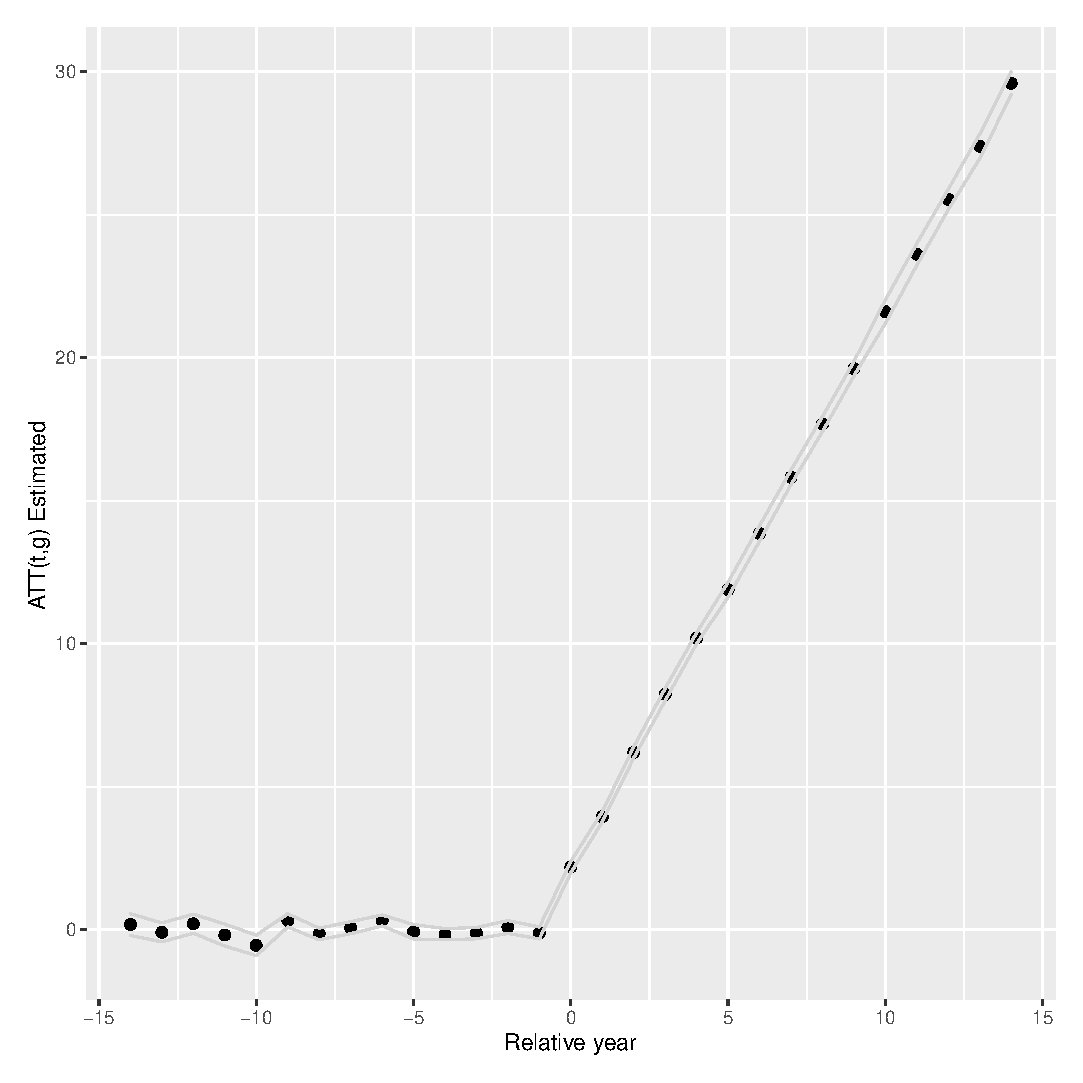
\includegraphics[width=0.7\textwidth]{fig/did_package_result.eps}
    \caption{$ATT(g,t)$ estimated by the \texttt{did} package. The ribbon represents $\pm 1 s.e$.}
\end{figure}

The slope is roughly 2, which matches the setting of our data generating process.